\documentclass[11pt]{article}

% --- Packages ---
\usepackage[utf8]{inputenc}
\usepackage[margin=1in]{geometry}
\usepackage{amsmath, amsthm, amssymb, amsfonts}
\usepackage{thmtools}
\usepackage{hyperref}
\usepackage{cleveref} % for referencing
\usepackage{booktabs}
\usepackage{bm} % for boldsymbol
\usepackage{graphicx}
\usepackage{float} % for images used inline
\usepackage{adjustbox}



% --- Theorem Environments ---
\declaretheoremstyle[headfont=\bfseries, bodyfont=\itshape]{mystyle}
\declaretheorem[style=mystyle, name=Theorem, numberwithin=section]{thm}
\declaretheorem[style=mystyle, name=Lemma, sibling=thm]{lem}
\declaretheorem[style=definition, name=Definition, sibling=thm]{defn}
\declaretheorem[style=remark, name=Remark, numbered=no]{rem}

% --- Custom Macros (Add your shortcuts here) ---
\newcommand{\R}{\mathbb{R}}
\newcommand{\Z}{\mathbb{Z}}
\newcommand{\norm}[1]{\left\lVert#1\right\rVert}

% --- Metadata ---
\title{Battery End of Life Predictions using Bayesian Hierarchical Modelling}
\author{Joshua Aziake, Mariam Elsayed}
\date{}

\begin{document}

\maketitle

\section{Introduction}

The lithium-ion battery is the predominant form of commercial rechargeable batteries, and are wildy used in many applications

Lithium-ion batteries are use in many wide spread applications, such as consumer electronics, toys, power tools, and electric vehicles

%However their performance degrades with time and usage \cite{HENDRICKS2015113}, remain difficult to understand since batteries are complex electrochemical devices that operate in widely varying conditions...

\section{Background}

The capacity of a lithium-ion battery --- the total charge deliverable in a full discharge --- fades 
with repeated cycling. With time and use, storage capacity diminishes and internal resistance increases, driven by 
degradation mechanisms that can occur simultaneously or trigger one another \cite{edge2021}. A battery is said to 
reach end-of-life (EoL) when its capacity drops below 80\% of its initial value, following the criterion used by 
Zhou et al.\ \cite{ZHOU20236117}.

The rate at which a battery charges or discharges is characterized by the C-rate, defined as the ratio of applied 
current to nominal capacity \cite{ossila_crate}. At 1C, a full charge or discharge completes in one hour; at 2C, 
in thirty minutes. Higher C-rates induce greater mechanical stress during cycling and promote lithium plating during 
charge \cite{edge2021}, both of which accelerate capacity fade. In the dataset used in this study, all cells are 
discharged at a fixed 4C rate while the charging protocol varies --- making the average charging C-rate the primary 
source of variability in operating conditions across cells.

\section*{Data Overview}
The primary data for this study is sourced from the comprehensive battery cycling datasets hosted on data.matr.io. The consolidated dataset consists of 169 Lithium-ion phosphate (LFP) cells cycled under varying fast-charging conditions. These cells represent 61 distinct average charging C-rates, providing various degradation profiles and cycle lifetimes.

\subsection*{Data Structure and Extraction}
The raw data, originally stored in MATLAB format, was ingested into a Python-based workflow for analysis. This process followed (authors and citation)'s process outlined in their GitHub. 
\begin{description}
    \item[Cell Level:] Each battery is indexed by a unique key. The keys map to a dictionary containing the \texttt{cycle\_life}, \texttt{charge\_policy}, \texttt{summary}, and \texttt{cycles}.
    \item[Summary Level:] High-level features are tracked each cycle, including Internal Resistance (IR), charge time, charge and discharge capacity ($Q_c$, $Q_d$), and temperature metrics ($T_{avg}$, $T_{min}$, $T_{max}$).
    \item[Cycle Level:] Time-series measurements within individual cycles provide charge and discharge capacity, linear interpolated discharge capacity, temperature, linear interpolated temperature, voltage, and derived vectors of discharge.
\end{description}

The \texttt{cycle\_life} indicates the number of cycles until end of life (EoL) is reached, while the \texttt{charge\_policy} indicates the specific charging protocol used for that cell.

\subsection*{Data Dictionary}

% Table 1: Cell Level
\begin{table}[h]
\centering
\caption{Cell Level Variables}
\label{tab:cell_level}
\begin{tabular}{lll}
\toprule
Variable & Description & Type \\
\midrule
\texttt{cycle\_life} & Number of cycles until EoL & Float \\
\texttt{charge\_policy} & Charging protocol & String \\
\texttt{summary} & Metadata for each cycle & Dictionary \\
\texttt{cycles} & Time series of measurements & Dictionary \\
\bottomrule
\end{tabular}
\end{table}

% Table 2: Summary Level
\begin{table}[h]
\centering
\caption{Summary Level (Cycle-by-Cycle Metadata)}
\label{tab:summary_level}
\begin{tabular}{lll}
\toprule
Variable & Description & Type \\
\midrule
\texttt{IR} & Internal resistance & Numeric array \\
\texttt{QC} & Charge capacity & Numeric array \\
\texttt{QD} & Discharge capacity & Numeric array \\
\texttt{Tavg} & Average temperature & Numeric array \\
\texttt{Tmin} & Minimum temperature & Numeric array \\
\texttt{Tmax} & Maximum temperature & Numeric array \\
\texttt{chargetime} & Charge time & Numeric array \\
\texttt{cycle} & Cycle number & Numeric array \\
\bottomrule
\end{tabular}
\end{table}

% Table 3: Cycle Level
\begin{table}[h!]
\centering
\caption{Cycle Level (Intra-cycle Time Series)}
\label{tab:cycle_level}
\begin{tabular}{lll}
\toprule
Variable & Description & Type \\
\midrule
\texttt{I} & Current & Numeric array \\
\texttt{Qc} & Charge capacity & Numeric array \\
\texttt{Qd} & Discharge capacity & Numeric array \\
\texttt{Qdlin} & Linear interpolated discharge capacity & Numeric array \\
\texttt{T} & Temperature & Numeric array \\
\texttt{Tdlin} & Linear interpolated temperature & Numeric array \\
\texttt{V} & Voltage & Numeric array \\
\texttt{dQdV} & Derived vectors of discharge & Numeric array \\
\texttt{t} & Time & Numeric array \\
\bottomrule
\end{tabular}
\end{table}

\subsection*{Data Partitioning and Grouping Logic}
Zhou and Howey (2023) partitioned the data into eight groups based on their cycling conditions and calculated the variance partition coefficient (VPC). Specifically, they calculated:

\begin{align*}
\text{VPC} &= \frac{\sigma^2_{\text{group}}}{\sigma^2_{\text{individual}} + \sigma^2_{\text{group}}} \\
\sigma^2_{\text{group}} &= \text{var}\left(\bar{u}_j - \bar{u}\right), \quad \bar{u} = \frac{1}{N} \sum_{j=1}^{k} \sum_{i=1}^{n_j} y_{ji} \\
\sigma^2_{\text{individual}} &= \text{var}\left(y_{ji} - \bar{u}_j\right), \quad \bar{u}_j = \frac{1}{n_j} \sum_{i=1}^{n_j} y_{ji}
\end{align*}

where $\sigma^2_{\text{group}}$ represents lifetime variance between groups and $\sigma^2_{\text{individual}}$ represents the total within-group lifetime variance. They obtained a VPC of 74.5\%, implying that between-group variance accounts for the majority of total lifetime variance. 

\subsection*{Grouping Results}
Following Zhou and Howey (2023), we first applied constrained K-means clustering on average charging C-rate. While this produced groups with low within-group C-rate variance (see Figure 1), the resulting VPC was only 38.973\%. We subsequently grouped cells by their unique charging policy string and optimized via a hill-climbing algorithm to achieve a VPC of 74.406\%. The hill-climb grouping exhibits higher within-group C-rate variance but lower within-group EoL variance (see Figure 2).

\begin{figure}[H]
    \centering
    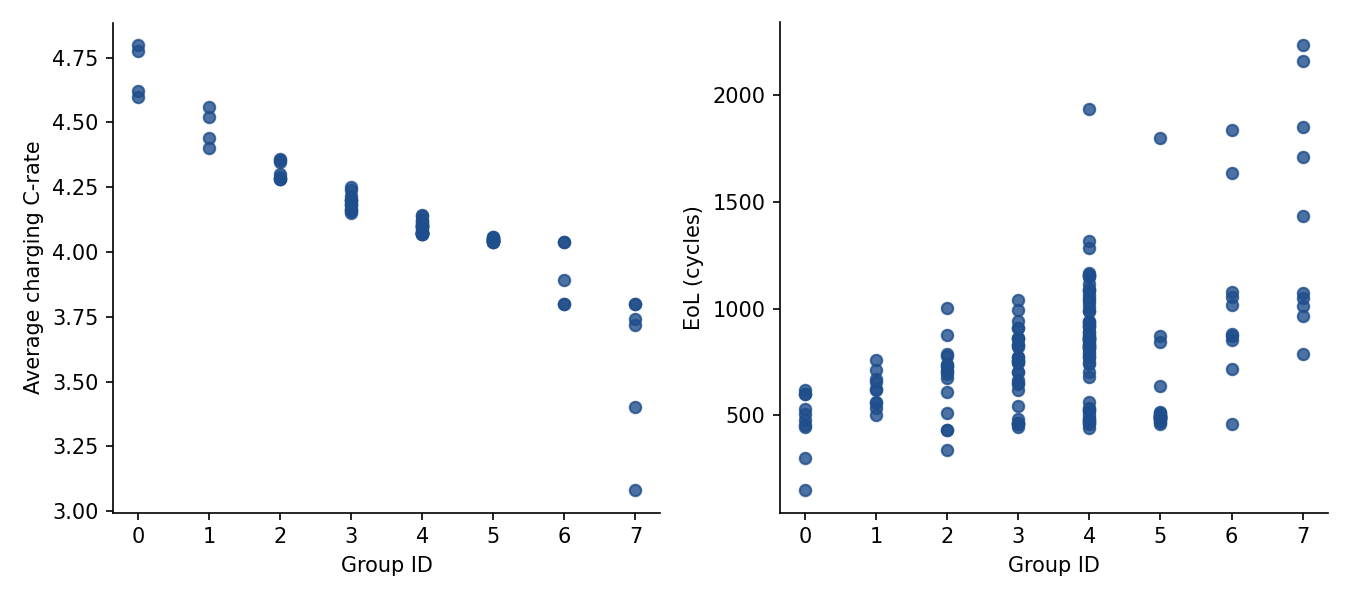
\includegraphics[width=0.8\textwidth]{fig4_km_group_crate_eol} 
    \caption{Distribution of average charging C-rate and EoL for each group obtained from constrained K-means.}
    \label{fig:battery_data}
\end{figure}
\begin{figure}[H]
    \centering
    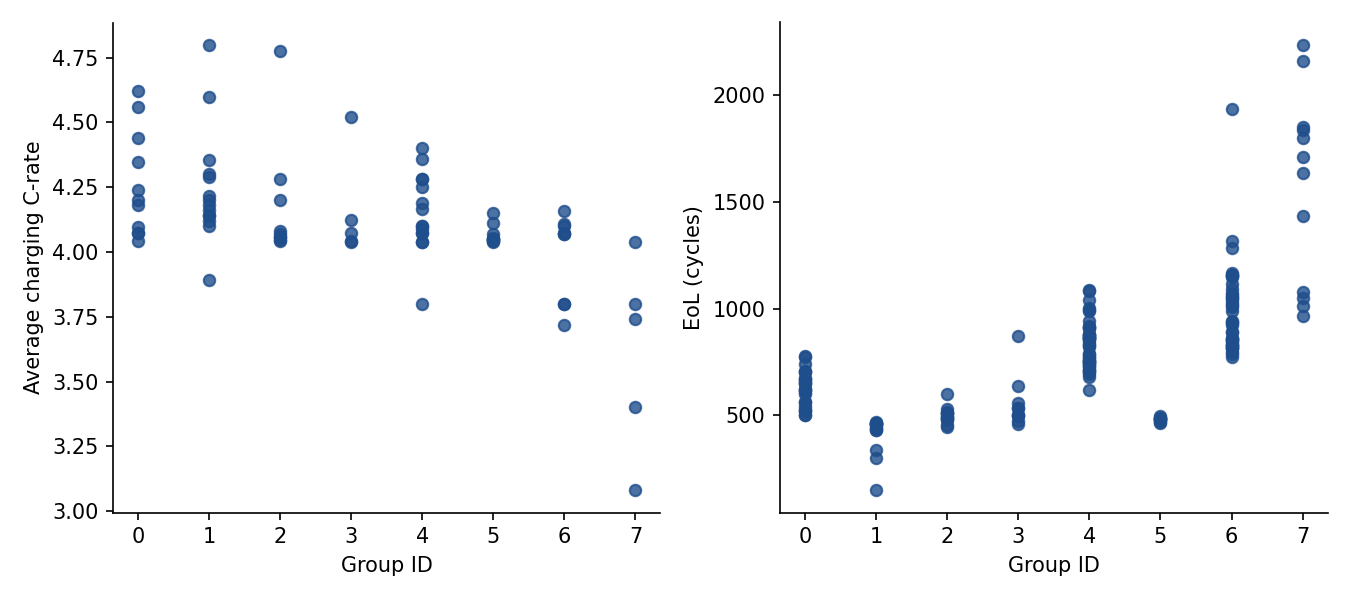
\includegraphics[width=0.8\textwidth]{fig4_group_crate_eol} 
    \caption{Distribution of average charging C-rate and EoL for each group obtained from hill-climb optimization.}
    \label{fig:battery_data}
\end{figure}

\section{Methodology}

\subsection{Bayesian Heirarchical Models}

A hierarchical model is a statistical model that includes multiple levels of parameters, where the parameters at one level are treated as random variables that depend on parameters at a higher level. In a Bayesian hierarchical model, we specify prior distributions for the parameters at each level, and use Bayes' theorem to update our beliefs about these parameters based on observed data.

We would like to capture both individual battery characteristics and the influence of different usage (cycling) conditions. A two level hierarchical structure is considered:
\begin{itemize}
    \item Level 1 (Cell-level parameters $\theta_j$): Each battery $j$ has its own parameters $\theta_j$ that represent how early cycle features relate to battery aging for that particular subgroup or cycling condition.
    \item Level 2 (Hyperparameters $\gamma$): These represent the parameters that govern the distribution of cell-level parameters across all subgroups, meaning they capture similarities across different batteries and cycling conditions.
\end{itemize}

Bayes rule is used to combine prior knowledge with the observed early-cycle data from multiple batteries to estimate posterior distributions of parameters at both levels. 

The level 2 posterior is calculated as 
$$
P(\gamma | \{Y\}) \propto \text{Likelihood} \times \text{Prior}
$$

\subsection{Multichain Monte Carlo}

\section{Experiment}

The analysis was completed in Python, and the hierarchical Bayesian model built in Python using the PyMC package \cite{pymc2023}. 

First, the data set was processed following section \ref{sec:dataoverview}. Early cycle features described in table \ref{table:features} were extracted and the data was partitioned into 8 groups like described in section \ref{subsec:GroupingResults}. The following experiment was completed using the grouping using the hill-climbing algorithm, because a high VPC justifies the use of a hierarchical model since group level effect would be significant. If the authors grouping method was used in this analysis with our data set, the VPC was only 39\% and the results of the hierarchical Baysian model would not be significantly.

The data was randomly split into a training and test dataset, with 135 cells in training set and 34 cell in the test set. The train-test split was stratified on the cycling group $g$, ensuring that the model will encounter the same proportions of cells from each cycling condition group. On the training set, a 5-fold cross validation was performed 4 times (so 20 results will be collected) to ensure that the model is not overfitting to the dataset. After that, the model was fit to the whole training set and evaluated using the unseen test set.

\section{Results and Discussion}

The performance of the Hierarchical Bayesian model is compared against two baselines: a ridge regression model with just the features in Table \ref{table:features}, and one including the cycling group $g$ as well. Root mean error squared (RMSE) and mean absolute percentage error (MAPE) are used as metrics to evaluate the performance of the models. We consider MAPE as an additional metric because RMSE is significantly influenced by outliers.
\begin{align*}
    \text{RMSE} &= \sqrt{\frac{\sum^N_{i=1} (y_i - \hat{y}_i)^2}{N}} \\
    \text{MAPE} &= \frac{1}{N}\sum^N_{i=1} \left| \frac{y_i - \hat{y}_i}{y_i} \right|
\end{align*}

\begin{table}[!ht]
\centering
\begin{tabular}{cccc}
\hline
             &   Baseline (without $g$) & Baseline (with $g$) &     HBM     \\
\hline
     RMSE    &    9.31                 &    6.51             &     7.23    \\
     MAPE    &    22.5\%                &    16.8\%           &     14.7\%  \\
\hline
\end{tabular}
\caption{Average RMSE (in days) and MAPE of the EoL predictions on the cross validation}
\label{table:RMSEandMAPE}
\end{table}

\begin{figure}[!ht]
    \centering
    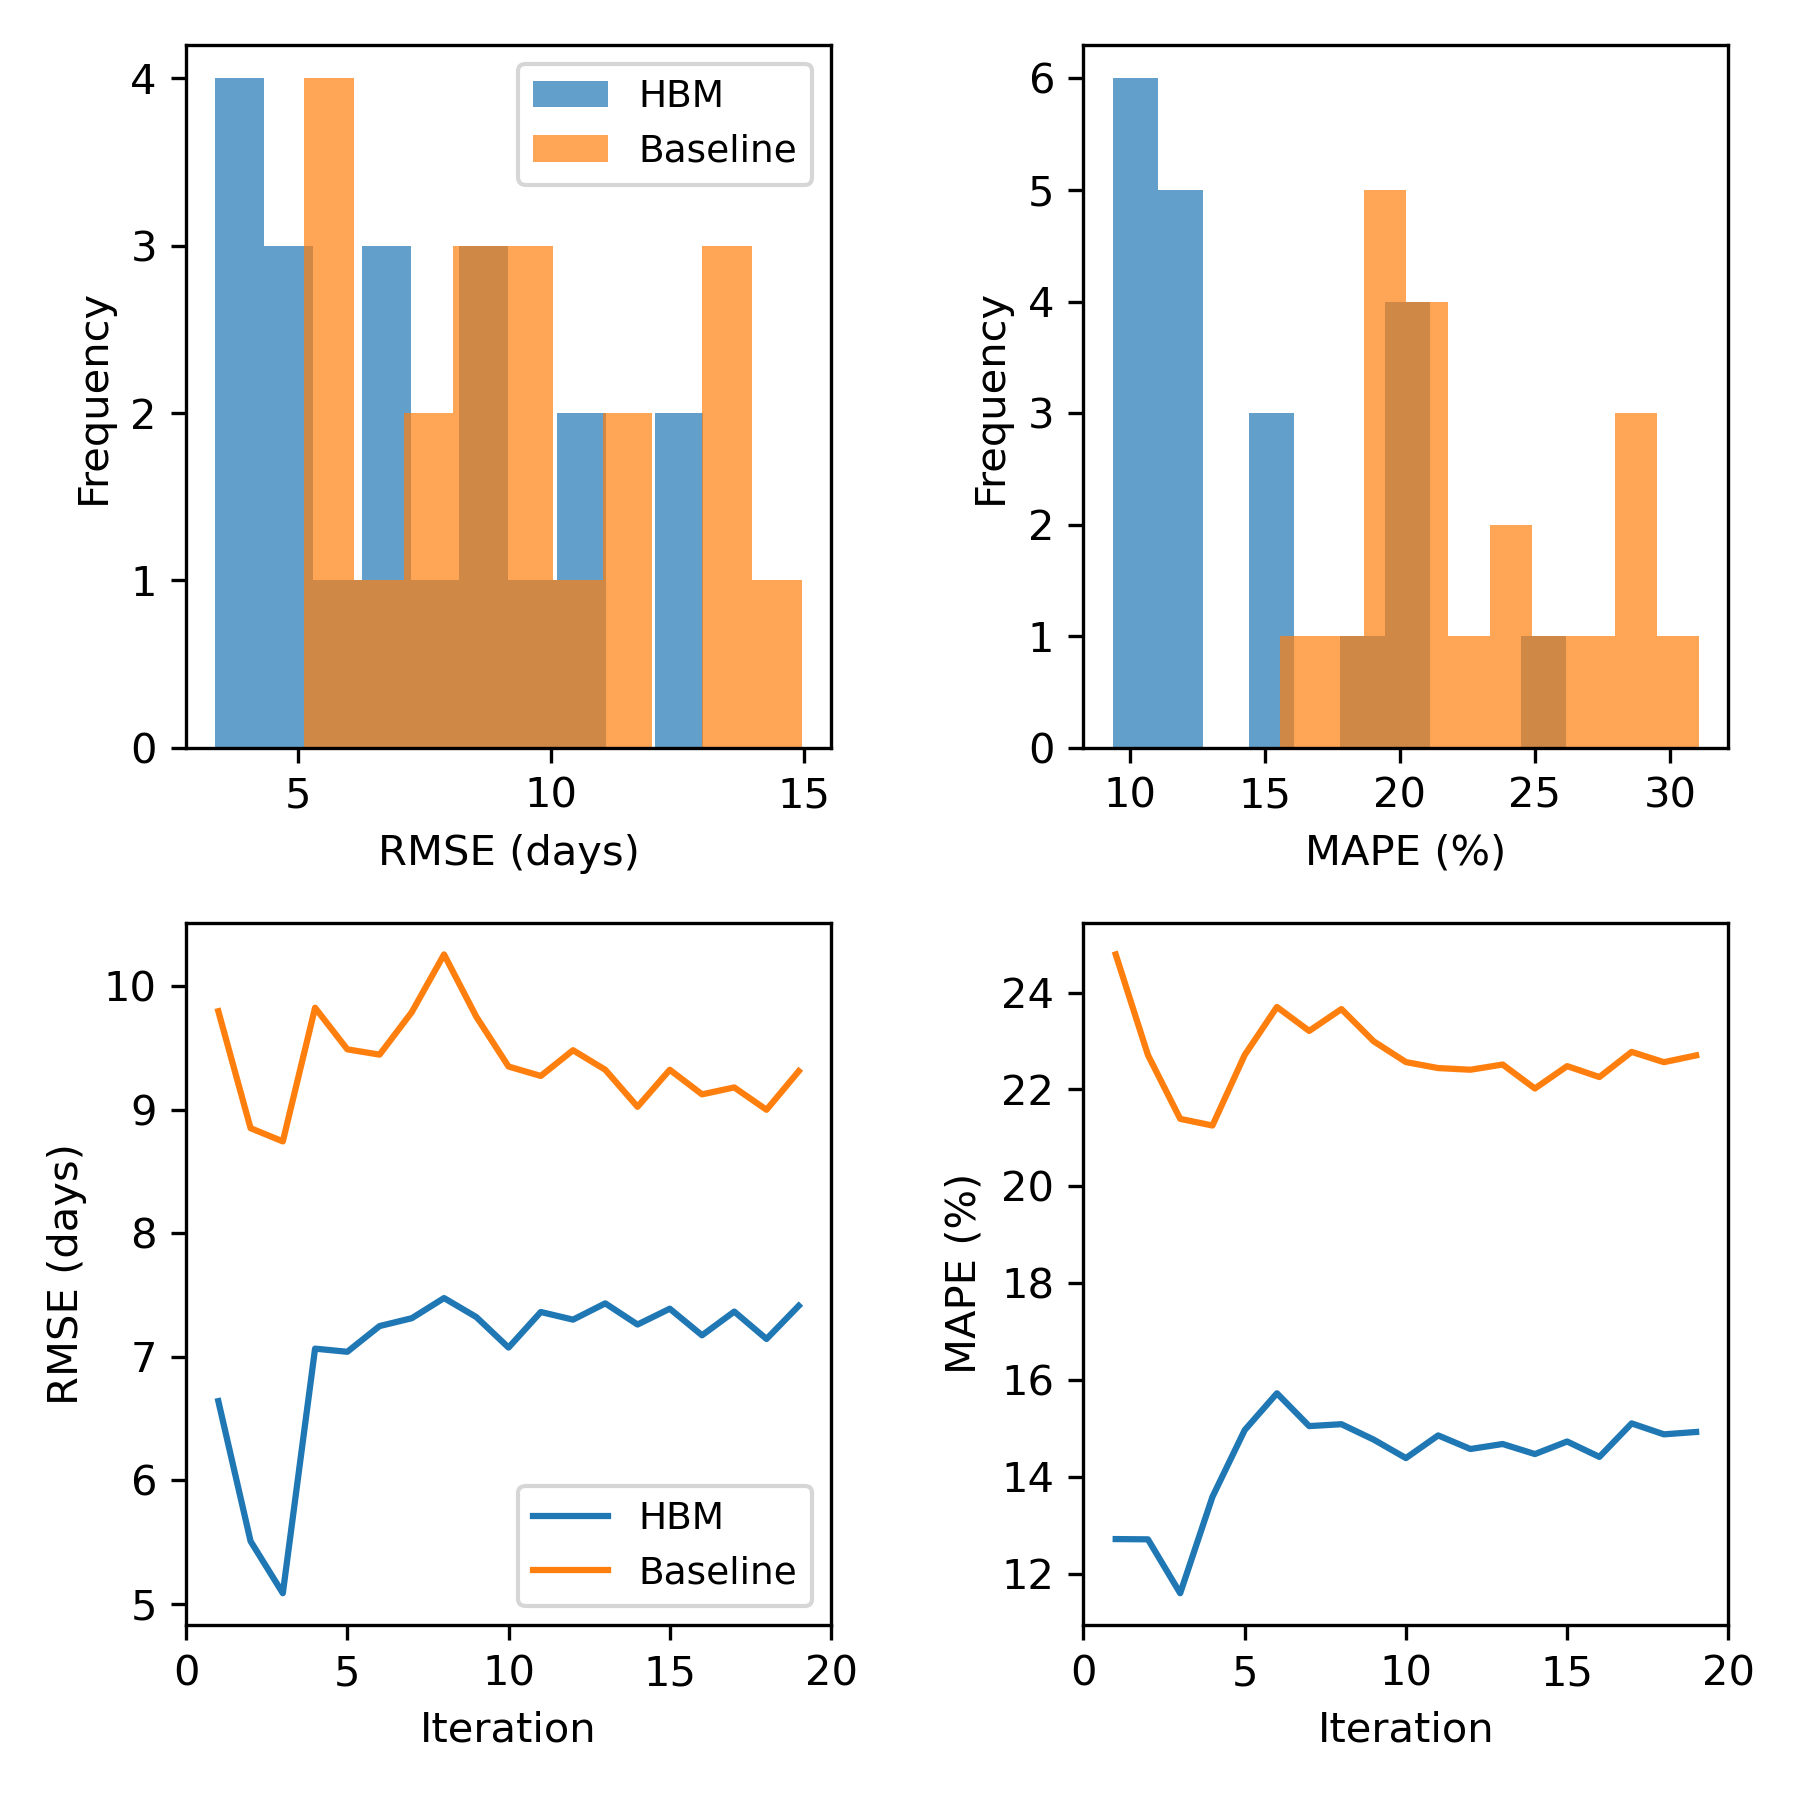
\includegraphics[width=0.75\linewidth]{kfolds_results.png}
    \caption{Histogram of all RSME and MAPE results for the HBM and baseline}
    \label{fig:kfolds_results}
\end{figure}

Table \ref{table:RMSEandMAPE} shows the average RMSE and MAPE after each repetition and fold, and figure \ref{fig:kfolds_results} shows the RMSE and MAPE values for each fold and repetition. HBM outperforms the baseline by $28.7\%$ with RMSE, but has similar results to the baseline with $g$ as a feature. This indicates the importance of the cycling condition as a feature and motivates the consideration of a hierarchical model, since conventional regression would treat the cycling condition and other features the same. Additionally, HBM outperforms both baseline models when considering MAPE. 

\begin{figure}[!ht]
    \centering
    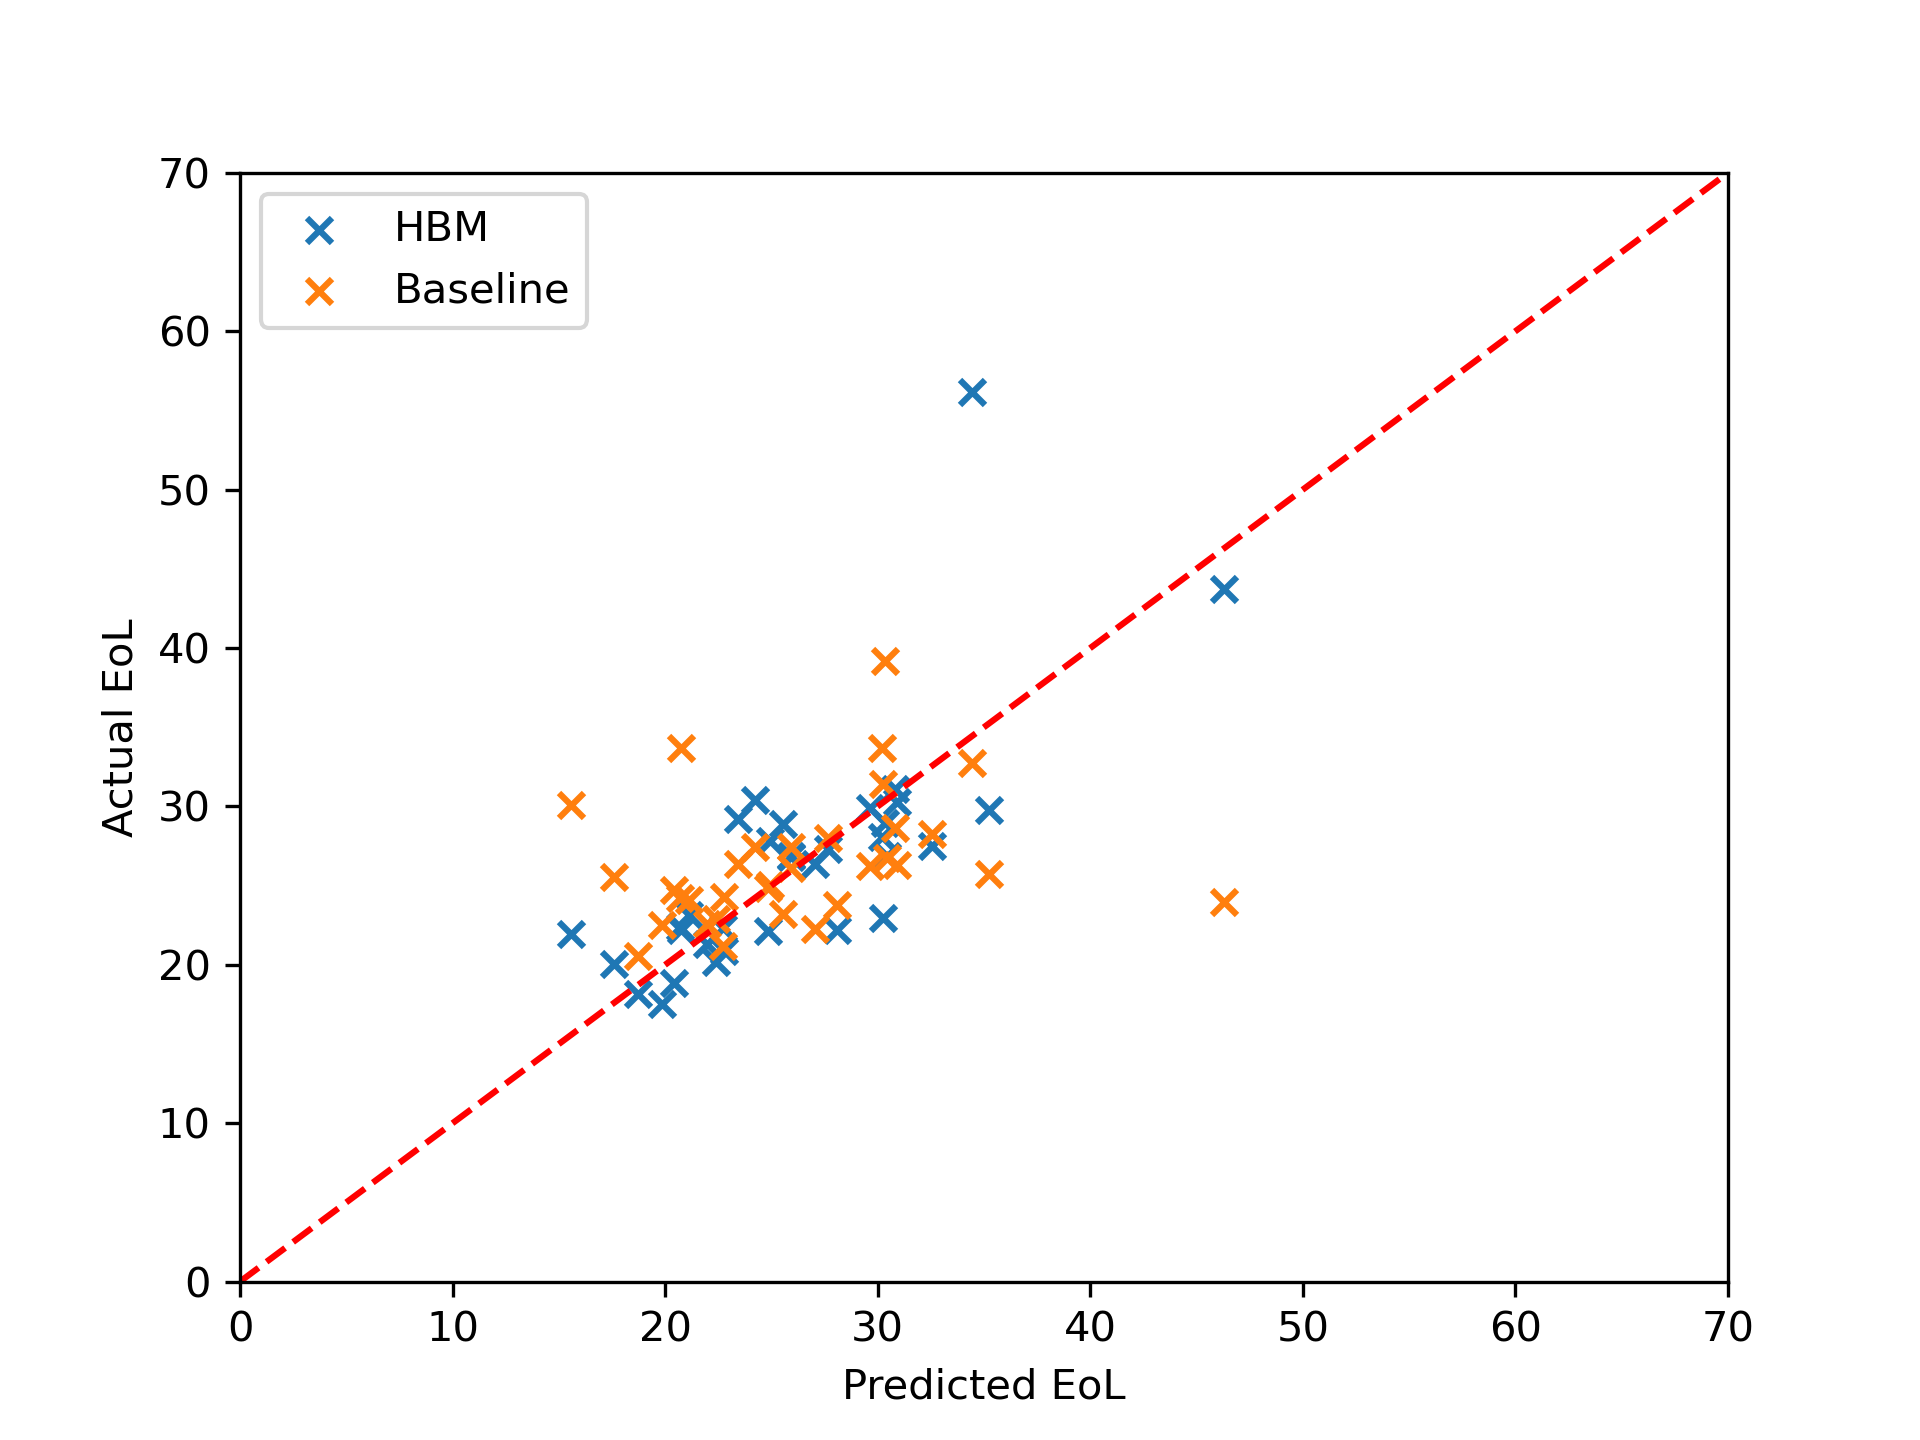
\includegraphics[width=0.75\linewidth]{results_scatterplot.png}
    \caption{Predicted v.s. actual EoL for HBM and baseline}
    \label{fig:results_scatterplot}
\end{figure}

\begin{table}[!ht]
\centering
\begin{tabular}{cccc}
\hline
             &   Baseline (without $g$) & Baseline (with $g$) &     HBM     \\
\hline
     RMSE    &    18.2                  &    18.2             &     18.8    \\
     MAPE    &    18.5\%                &    17.1\%           &     13.9\%  \\
\hline
\end{tabular}
\caption{RMSE (in days) and MAPE of the EoL predictions on the test set}
\label{table:finalRMSEandMAPE}
\end{table}

Now using just a training and test set, table \ref{table:finalRMSEandMAPE} shows the RMSE and MAPE on the test set predictions and figure \ref{fig:results_scatterplot} shows the EoL predictions from the HBM and baseline models compared to the true values.

\section{Conclusion}

This work investigated the use of a hierarchical Bayesian model (HBM) for predicting battery end-of-life (EoL) from early-cycle features, incorporating cycling condition as a group-level structure rather than a flat input feature. Three early-cycle features were extracted following the approach of \cite{severson2019}, and cells were partitioned into 8 groups based on charging protocol using a hill-climbing algorithm, which produced a variance partition coefficient sufficient to justify a hierarchical treatment of the data.

Across 20 cross-validation folds, the HBM achieved a mean MAPE of $14.7\%$, outperforming both the plain ridge baseline ($22.5\%$) and the ridge model with the group feature ($16.8\%$). On the held-out test set, the HBM maintained the lowest MAPE at $13.9\%$, though its RMSE was marginally higher than the baselines, suggesting sensitivity to a small number of outlier predictions. MCMC diagnostics confirmed reliable posterior inference, with all parameters satisfying $\hat{R} \leq 1.01$ and adequate effective sample sizes.

Bayesian posterior analysis revealed that the hyperprior slope linking mean C-rate to the group intercept was credibly negative (HDI $[-4.91, -1.55]$), providing probabilistic evidence that higher charge rates are associated with reduced battery lifetime at the group level. The early-cycle feature coefficients, by contrast, were found to generalize across groups, with no credible C-rate modulation. Together, these findings suggest that the performance advantage of the HBM over conventional regression stems not from learning different feature sensitivities per group, but from appropriately pooling information across cells sharing similar cycling conditions when estimating baseline lifetime.

Future work could explore richer group structures and the influence of cluster size and number. The grouping of the cycling conditions heavily influenced the results of HBM as well as the baseline rigde regression with the group feature.

\clearpage
\bibliographystyle{plain} 
\bibliography{refs} 

\clearpage
\appendix
\section*{Appendix}


\subsection*{Data Dictionary}

% Table 1: Cell Level
\begin{table}[H]
\centering
\caption{Cell Level Variables}
\label{tab:cell_level}
\begin{tabular}{lll}
\toprule
Variable & Description & Type \\
\midrule
\texttt{cycle\_life} & Number of cycles until EoL & Float \\
\texttt{charge\_policy} & Charging protocol & String \\
\texttt{summary} & Metadata for each cycle & Dictionary \\
\texttt{cycles} & Time series of measurements & Dictionary \\
\bottomrule
\end{tabular}
\end{table}

% Table 2: Summary Level
\begin{table}[H]
\centering
\caption{Summary Level (Cycle-by-Cycle Metadata)}
\label{tab:summary_level}
\begin{tabular}{lll}
\toprule
Variable & Description & Type \\
\midrule
\texttt{IR} & Internal resistance & Numeric array \\
\texttt{QC} & Charge capacity & Numeric array \\
\texttt{QD} & Discharge capacity & Numeric array \\
\texttt{Tavg} & Average temperature & Numeric array \\
\texttt{Tmin} & Minimum temperature & Numeric array \\
\texttt{Tmax} & Maximum temperature & Numeric array \\
\texttt{chargetime} & Charge time & Numeric array \\
\texttt{cycle} & Cycle number & Numeric array \\
\bottomrule
\end{tabular}
\end{table}

% Table 3: Cycle Level
\begin{table}[H]
\centering
\caption{Cycle Level (Intra-cycle Time Series)}
\label{tab:cycle_level}
\begin{tabular}{lll}
\toprule
Variable & Description & Type \\
\midrule
\texttt{I} & Current & Numeric array \\
\texttt{Qc} & Charge capacity & Numeric array \\
\texttt{Qd} & Discharge capacity & Numeric array \\
\texttt{Qdlin} & Linear interpolated discharge capacity & Numeric array \\
\texttt{T} & Temperature & Numeric array \\
\texttt{Tdlin} & Linear interpolated temperature & Numeric array \\
\texttt{V} & Voltage & Numeric array \\
\texttt{dQdV} & Derived vectors of discharge & Numeric array \\
\texttt{t} & Time & Numeric array \\
\bottomrule
\end{tabular}
\end{table}

\subsection*{Model Variables and Features}


\begin{table}[H]
\centering
\caption{Variables}
\begin{tabular}{ll}
\toprule
Symbol & Description \\
\midrule
$j = 1, \dots, J$ & Cycling condition group index \\
$i = 1, \dots, n_j$ & Cell index within group $j$ \\
$y_{ji}$ & EoL time (days) for cell $i$ in group $j$ \\
$\boldsymbol{\theta}_j \in \mathbb{R}^4$ & Regression coefficients for group $j$ \\
$\sigma^2_j$ & Variance of group $j$ model \\
$\boldsymbol{\gamma} \in \mathbb{R}^{4 \times 2}$ & Hyperparameter matrix linking cycling conditions to group coefficients \\
\bottomrule
\end{tabular}
\end{table}

\begin{table}[H]
\centering
\caption{Feature vectors}
\begin{tabular}{lll}
\toprule
Symbol & Components & Level \\
\midrule
$\mathbf{x}_{ji} \in \mathbb{R}^4$ & $(1, F1_{ji}, F2_{ji}, F3_{ji})^\top$ & Individual \\
$\mathbf{g}_j \in \mathbb{R}^2$ & $(1, \bar{g}_j)^\top$ & Group \\
\bottomrule
\end{tabular}
\end{table}

\begin{table}[H]
\centering
\caption{Individual-level features (computed from first 100 cycles)}
\begin{tabular}{ll}
\toprule
Symbol & Description \\
\midrule
$F1_{ji}$ & Variance of $\Delta Q(V)$ between cycles 10 and 100 \\
$F2_{ji}$ & Minimum of $\Delta Q(V)$ over the same interval \\
$F3_{ji}$ & Discharge capacity at cycle 2 \\
\bottomrule
\end{tabular}
\end{table}
\footnote{$\Delta Q(V)$ denotes the discharge curve difference as a function of voltage, following Severson et al. (2019).}


\end{document}